\documentclass[10pt,a4paper]{article}
\usepackage[margin=22mm]{geometry}
\usepackage[T1]{fontenc}
\usepackage{lmodern,microtype,amsmath,amssymb,booktabs,tabularx,array,longtable}
\usepackage{graphicx,xcolor,tikz,pgfplots,caption,float,placeins}
\usepackage[hidelinks]{hyperref}
\usetikzlibrary{arrows.meta,positioning,fit,backgrounds,calc}
\pgfplotsset{compat=1.18}
\definecolor{ariaBlue}{HTML}{235789}
\definecolor{ariaTeal}{HTML}{267A73}
\definecolor{ariaGold}{HTML}{956B23}
\definecolor{ariaGray}{HTML}{526170}
\captionsetup{font=small,labelfont=bf,skip=7pt}
\setlength{\parskip}{3pt}
\setlength{\parindent}{12pt}
\setlength{\emergencystretch}{2em}
\renewcommand{\arraystretch}{1.15}
\newcolumntype{Y}{>{\raggedright\arraybackslash}X}
\newcommand{\source}[1]{\par\smallskip{\footnotesize\emph{Source and scope:} #1}}
\tikzset{box/.style={draw=ariaBlue,fill=ariaBlue!5,rounded corners=2pt,align=center,minimum height=12mm,text width=39mm,font=\small,inner sep=4pt},arr/.style={-{Latex[length=2mm]},thick,draw=ariaGray},pending/.style={box,draw=ariaGold,dashed,fill=ariaGold!6}}
\title{\textbf{ARIA: A Belief-Aware Architecture for Adaptive Mock Interviews\\with Multimodal Baseline Evaluation}}
\author{Raghav Samir Sejpal \and Krissh Verma}
\date{School of Computer Science and Engineering\\Vellore Institute of Technology, Vellore, Tamil Nadu, India}
\begin{document}
\maketitle
\begin{abstract}
An adaptive mock interviewer must decide what to ask next from evidence that is incomplete and sometimes unreliable. A useful design therefore needs both a representation of what has been learned and an evaluation that distinguishes response scoring from question-selection quality. We present ARIA, an Autonomous Reinforcement-Based Interview Agent that combines role-grounded questions, calibrated skill beliefs, and an offline Implicit Q-Learning policy. The current policy interface uses a 33-dimensional state and eight actions. We bring together recorded component benchmarks, a locked synthetic belief evaluation, and matched development rollouts against behavior cloning, discrete Conservative Q-Learning, and Decision Transformer adaptations. The component records show that TF-IDF with a linear SVM achieved macro-F1 of 0.6030 on short-answer grading, while text-only CMU-MOSEI accuracy of 0.8015 slightly exceeded early fusion at 0.7976. On 91 locked-test episodes, the calibrated belief model achieved accuracy of 0.9121 and macro-F1 of 0.9168. In 45 matched development rollouts per condition, base accuracy saturated across several policies. Under overlapping evidence, ARIA IQL achieved accuracy 0.4667, while behavior cloning achieved 0.5333; however, IQL obtained the largest mean designed reward and information gain among the learned comparators in every evaluated condition. The comparison therefore supports a claim about simulator behavior, not superior assessment accuracy or real-candidate performance. Live policy integration and human validation remain necessary.
\end{abstract}
\noindent\textbf{Keywords:} adaptive mock interviews; multimodal learning; baseline comparison; belief calibration; implicit Q-learning; offline reinforcement learning.

\section{Introduction}
A useful practice interview responds to what a candidate has actually said. A weak answer may justify a simpler question, an incomplete explanation may call for a follow-up, and a well-supported answer may allow the interviewer to move to another topic. Implementing these choices requires more than a fluent question generator. The system must retain evidence across turns, recognize uncertainty, and distinguish a change in question difficulty from a change in its estimate of the candidate's knowledge.

Automated interview research has approached this problem from several directions. HireNet models the hierarchy of questions and answers to predict recruiter judgments from recorded interviews \cite{hirenet}. More recent platforms, such as PolyInterview, combine role-specific questions, spoken interaction, and multimodal feedback \cite{poly}. Adaptive testing offers a complementary view: the next item is selected because of what it can reveal about an uncertain latent trait \cite{cat}. These approaches establish useful precedents, but their evaluation targets differ. A model that predicts a rating, a system that produces relevant questions, and a policy that improves the evidence collected during an interview answer different research questions.

ARIA studies the connection between evidence accumulation and action selection. It represents skill estimates as probability distributions and exposes a fixed interface through which a policy can change topic, probe foundations, adjust difficulty, or end an interview. The offline learner is trained on synthetic trajectories, while separate component experiments examine visual emotion recognition, speech emotion classification, short-answer grading, sentiment fusion, and an annotated deception task. These component tasks provide engineering evidence about candidate modules. They do not turn emotion or deception labels into validated measures of interview competence.

The evaluation is organized around three questions. First, what do the available baseline experiments reveal about the usefulness of the proposed components? Second, does the current calibration improve belief estimates on a held-out synthetic set? Third, what evidence connects those estimates to the behavior of an adaptive interview policy? This organization allows positive findings to be stated directly while making clear where the evidence stops.

The study contributes a code-grounded account of the belief-to-action architecture, a consolidated analysis of previously scattered baseline results, and a paired evaluation of the current belief model. It also positions the system against contemporary work without treating scores from different datasets as a common leaderboard. The strongest present result concerns synthetic belief estimation. The complete architecture remains a research prototype for mock-interview experimentation.

\section{Related work and state-of-the-art analysis}
\subsection{From interview scoring to interactive practice}
HireNet treats an interview as a sequence of question--answer pairs and uses hierarchical attention to model context \cite{hirenet}. Its target is a recruiter-provided hirability judgment. This is a relevant precedent for representing interview evidence, although it does not evaluate ARIA's eight-action policy. PolyInterview moves closer to the interaction problem by conditioning questions on a CV and job description, asking answer-aware follow-ups, and linking feedback to multimodal observations \cite{poly}. Its existence means that adaptation and multimodal feedback alone cannot serve as ARIA's distinguishing contribution.

The distinction is clearer when the system is viewed as an experimental interface. ARIA exposes the state used for action selection, the conditions under which a belief can be reported, and the provenance of the frozen evaluation. Researchers can then ask whether a changed component alters belief quality or policy behavior. Inspectability is an engineering property; it is not evidence of superior interviewing performance.

\subsection{Multimodal prediction and the value of additional signals}
Multimodal assessment is useful only when an added signal contributes information relevant to the intended target. Kim et al. address fairness in automated video interview assessment through distributional regularization, with a tunable accuracy--fairness trade-off \cite{kim}. MAG-BERT-ARL combines a multimodal language representation with adversarial reweighting to address underrepresented groups without relying on sensitive attributes \cite{mag}. These studies treat fairness as an evaluation objective rather than a consequence of adding more modalities.

AVI-Personality provides a recent dataset built around trait-targeted interview questions and labels reported by participants and observers. Its benchmarks find strong text baselines and only modest overall gains from multimodal methods \cite{avi}. For ARIA, the relevant implication is methodological: each modality should be compared against a text baseline under the same split and outcome definition. The local fusion results examined below make this requirement concrete. A visually elaborate architecture should not obscure a simpler model that performs as well or better.

\subsection{Adaptive assessment and offline learning}
Deep computerized adaptive testing combines multivariate latent-trait modeling with learned item selection \cite{cat}. Its testing setting differs from open-ended interviews, but it supports treating question selection as a sequential decision problem rather than a fixed script. In ARIA, the policy acts on an explicit summary of beliefs, coverage, and recent evidence.

Implicit Q-Learning provides the algorithmic basis for the offline policy \cite{iql}. Its advantage-weighted policy extraction and expectile value learning reduce the need to query unsupported actions during training. Conservative Q-Learning instead regularizes learned action values to reduce overestimation outside the logged distribution \cite{cql}. Decision Transformer frames offline control as return-conditioned causal sequence modeling over states, actions, and rewards \cite{decisiontransformer}. These methods provide relevant same-data architectures, but their original benchmark scores are not directly comparable with ARIA. Off-policy evaluation addresses a separate question: how much can be inferred about a new policy from data collected by another policy? Work on high-confidence evaluation makes the distinction between a point estimate and a defensible performance bound explicit \cite{ope}.

\subsection{Comparative position of ARIA}
Table~\ref{tab:sota} compares representative contemporary systems and methodological precedents. Here, state-of-the-art analysis means an assessment of relevant approaches and their evidence, not a claim that ARIA has achieved the best published score. The comparison is selective and includes 2026 preprints; publication status is retained because the level of external review differs across sources.

\begin{table}[htbp]
\centering\small
\caption{State-of-the-art analysis by task and evaluation target. No row is a direct numerical competitor to ARIA's synthetic belief test.}
\label{tab:sota}
\begin{tabularx}{\linewidth}{p{27mm}YYY}
\toprule
Work & Main approach & Evidence or target & Relationship to ARIA \\ \midrule
HireNet (2019) \cite{hirenet} & Hierarchical attention over recorded interviews & Recruiter hirability judgments & Representation precedent; different labels and no shared policy test \\
Kim et al. (2023) \cite{kim} & Fairness-aware multimodal learning & Predictive scores and fairness trade-offs & Establishes the need to measure group effects separately \\
MAG-BERT-ARL (2024) \cite{mag} & Multimodal language model with adversarial reweighting & Performance and fairness on interview-related datasets & Fairness comparator; not reproduced in this study \\
Deep CAT (2026) \cite{cat} & Multivariate trait estimation and learned item selection & Simulated and real assessment data & Sequential-assessment precedent; different item and response setting \\
PolyInterview (2026 preprint) \cite{poly} & Role-conditioned dialogue and multimodal feedback & Platform use, question alignment, expert assessment & Close systems comparator; ARIA's contribution must be narrower than adaptation \\
AVI-Personality (2026 preprint) \cite{avi} & Trait-activated multimodal interview dataset & Reliability, validity, fairness, predictive benchmarks & Future external-validation resource; not an ARIA evaluation dataset \\
ARIA (this study) & Calibrated belief state and offline IQL interface & Locked beliefs and matched synthetic development rollouts & Inspectable integration design; real-candidate policy effectiveness remains open \\
\bottomrule
\end{tabularx}
\end{table}

\section{Problem formulation and architecture}
\subsection{Interview state and decision objective}
Let $o_t$ denote the response evidence available after turn $t$. For each skill $k$, ARIA maintains a three-class belief $b_{k,t}$ over beginner, intermediate, and expert levels. These are operational categories in the synthetic evaluation. They should not be read as validated occupational qualifications. The policy receives a summary $s_t=\phi(b_t,h_t,m_t)$, where $h_t$ contains recent interaction history and $m_t$ indicates which evidence channels are available.

The sequential objective is
\begin{equation}
J(\pi)=\mathbb{E}_{\tau\sim\pi}\left[\sum_{t=0}^{T-1}\gamma^t r_t\right],\qquad \gamma=0.99.
\end{equation}
Here, $r_t$ is a designed simulation reward. It is distinct from a human judgment of interview quality. A policy can optimize this objective only to the extent that the reward and environment represent the intended behavior. The historical simulations and the current offline diagnostic use different evidence streams, so their reward numbers are not combined.

\subsection{System overview}
Figure~\ref{fig:architecture} separates context construction, evidence processing, and sequential decision making. Resume and job-description context define the skill space. Response-processing modules can provide semantic, acoustic, and visual observations, while availability indicators allow missing channels to remain visible. The current belief update uses semantic evidence and confidence factors; the behavioral score is accepted by the function interface for compatibility but does not enter its competency likelihood.

\begin{figure}[htbp]
\centering
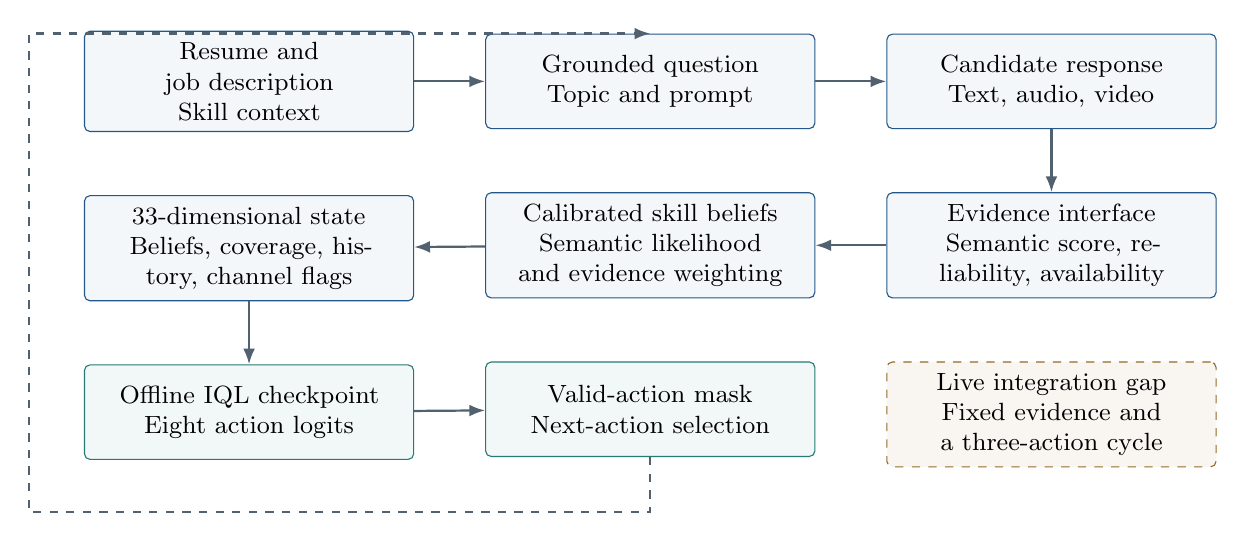
\begin{tikzpicture}[node distance=8mm and 9mm]
\node[box] (context) {Resume and job description\\Skill context};
\node[box,right=of context] (question) {Grounded question\\Topic and prompt};
\node[box,right=of question] (answer) {Candidate response\\Text, audio, video};
\node[box,below=of answer] (evidence) {Evidence interface\\Semantic score, reliability, availability};
\node[box,below=of question] (belief) {Calibrated skill beliefs\\Semantic likelihood and evidence weighting};
\node[box,below=of context] (state) {33-dimensional state\\Beliefs, coverage, history, channel flags};
\node[box,below=of state,draw=ariaTeal,fill=ariaTeal!6] (policy) {Offline IQL checkpoint\\Eight action logits};
\node[box,below=of belief,draw=ariaTeal,fill=ariaTeal!6] (mask) {Valid-action mask\\Next-action selection};
\node[pending,below=of evidence] (live) {Live integration gap\\Fixed evidence and a three-action cycle};
\draw[arr] (context)--(question);\draw[arr] (question)--(answer);
\draw[arr] (answer)--(evidence);\draw[arr] (evidence)--(belief);
\draw[arr] (belief)--(state);\draw[arr] (state)--(policy);
\draw[arr] (policy)--(mask);
\draw[arr,dashed] (mask.south)--++(0,-7mm)-| ([xshift=-7mm]context.west)|-(question.north);
\end{tikzpicture}
\caption{ARIA's intended decision loop and current implementation boundary. Solid arrows show component data dependencies; the dashed return path denotes the intended learned-policy control loop. The live application does not yet execute that loop. Acoustic and visual channels are candidate contextual inputs, not validated skill measurements.}
\label{fig:architecture}
\end{figure}

The architecture therefore has two implementation levels. The offline pipeline contains the calibrated belief configuration, trajectory reconstruction, a trained policy, and provenance checks. The live application supports question and response interaction, but currently supplies semantic and behavioral values of 0.9, assigns low cognitive load, and cycles through foundation probing, increased difficulty, and topic switching. An inference module for the IQL checkpoint exists; its existence does not mean the application invokes it. Keeping this distinction in the architecture prevents an interface demonstration from being mistaken for an end-to-end policy experiment.

\subsection{The 33-dimensional state}
Table~\ref{tab:state} follows the ordered feature contract in the current state builder. Aggregating skill beliefs avoids a state size that depends on the number or order of ontology nodes. The focused skill still has its own three-class distribution, allowing the policy to distinguish uncertainty about the present topic from uncertainty about the interview as a whole.

\begin{table}[htbp]
\centering\small
\caption{State groups in the current implementation. The valid-action mask is supplied separately.}
\label{tab:state}
\begin{tabularx}{\linewidth}{Y r Y}
\toprule Group & Dimensions & Contents \\ \midrule
Global belief and uncertainty & 5 & Three aggregate probabilities; assessment and mean visited-skill entropy \\
Session progress & 3 & Skill coverage, turn fraction, valid-evidence fraction \\
Focused skill & 5 & Three probabilities, effective evidence, consecutive-focus fraction \\
Recent evidence & 8 & Semantic score, reliability, behavior score, four cognitive-label indicators, incongruence score \\
Previous action & 8 & One-hot representation of the preceding action \\
Evidence availability & 4 & Semantic, behavioral, cognitive, and incongruence flags \\
\midrule Total & 33 & Fixed ordered representation, \texttt{aria-state-v4} \\
\bottomrule
\end{tabularx}
\end{table}

Progress variables and effective evidence are bounded before entering the policy. The representation includes a previous-action encoding, while the action mask identifies choices that are currently legal. For example, concluding can be disallowed until the environment's stopping conditions are met. The eight actions are increasing difficulty, decreasing difficulty, following up on the same topic, switching topic, probing foundations, asking a behavioral question, asking a situational question, and concluding. A policy action specifies the interview move; the question generator supplies the corresponding wording.

\subsection{Belief update and decision calibration}
For semantic score $x_t$ and class $c$, the implemented log-likelihood has the form
\begin{equation}
\ell_c(x_t)=-\frac{1}{2}\left(\frac{x_t-\mu_c}{\sigma_c}\right)^2-\log\sigma_c.
\end{equation}
The update is a reliability-weighted change in log probability:
\begin{equation}
b_{k,t+1}(c)\propto b_{k,t}(c)\exp\{w_t\ell_c(x_t)\}.
\end{equation}
The weight $w_t$ combines evidence, transcription, and modality confidence. It is discounted as effective evidence accumulates, reduced for a repeated question fingerprint, and capped by the remaining evidence allowance for that skill. Normalization and a posterior floor keep the distribution usable. These operations limit the influence of repeated or unreliable evidence without treating a missing observation as a negative answer.

The aggregate belief uses a normalized log-opinion pool over visited skills. Skill importance and capped effective evidence determine the pooling weights. A temperature parameter adjusts the aggregate distribution. The current belief schema also supports a beginner-class logit bias, applied before confidence and the final decision are calculated. This cost-sensitive adjustment should be distinguished from probability calibration: an improved classification boundary can coexist with a worse calibration metric.

A label is returned only when confidence, effective evidence, and visited-skill coverage satisfy their configured requirements. Otherwise, the output is insufficient evidence. All locked-test episodes were classified in the recorded evaluation; this observation does not imply that abstention is disabled in the implementation.

\subsection{Offline IQL training and inference}
The implementation contains a value network, two Q-functions, and a categorical policy network. Each uses two hidden layers of 256 units, layer normalization, ReLU activations, and dropout of 0.1. Q-functions receive the state and one-hot action; the policy produces eight action logits. Following IQL \cite{iql}, the value objective uses an asymmetric squared error,
\begin{equation}
L_V=\mathbb{E}_{(s,a)\sim D}\left[|\tau-\mathbb{1}(u<0)|u^2\right],\quad u=\min_j\bar Q_j(s,a)-V(s),
\end{equation}
with expectile $\tau=0.8$. The Q-functions fit the target $r+\gamma(1-d)V(s')$, where $d$ indicates termination. Policy extraction minimizes
\begin{equation}
L_\pi=-\mathbb{E}_{(s,a)\sim D}\left[\min\{e^{\beta A(s,a)},100\}\log\pi(a\mid s)\right],\quad \beta=3.
\end{equation}
These equations describe the current training code. They do not define a new offline RL algorithm. At inference, schema checks validate the feature order and checkpoint provenance, and action masking removes illegal choices before selection.

\section{Experimental design and evidence provenance}
\subsection{Three evaluation streams}
The repository contains results produced at different stages of development. Figure~\ref{fig:evidence} shows how they are used. Component benchmark summaries provide recorded results for candidate modules. A separate 300-episode simulation compares five historical policies. The current release provides machine-readable belief and policy-diagnostic reports. Only the last stream is tied to the frozen v7 belief configuration and current IQL checkpoint.

\begin{figure}[htbp]
\centering
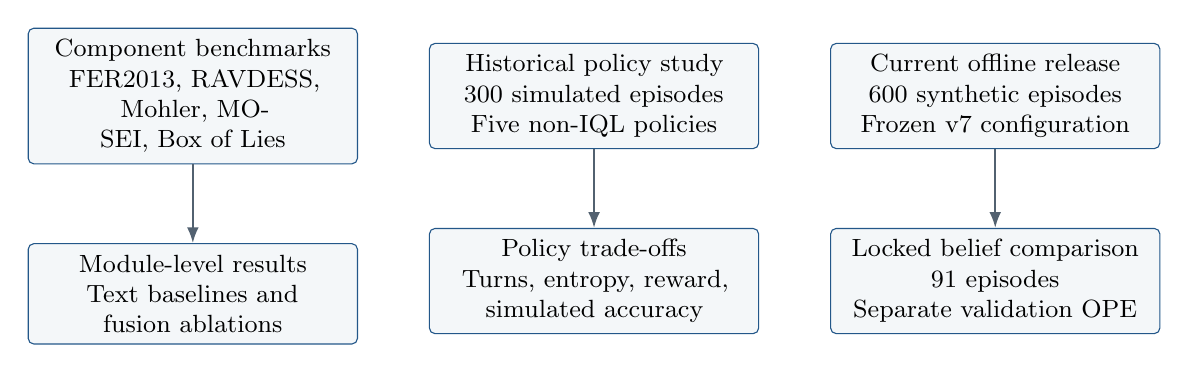
\begin{tikzpicture}[node distance=10mm and 9mm]
\node[box] (a) {Component benchmarks\\FER2013, RAVDESS, Mohler, MOSEI, Box of Lies};
\node[box,right=of a] (b) {Historical policy study\\300 simulated episodes\\Five non-IQL policies};
\node[box,right=of b] (c) {Current offline release\\600 synthetic episodes\\Frozen v7 configuration};
\node[box,below=of a] (aa) {Module-level results\\Text baselines and fusion ablations};
\node[box,below=of b] (bb) {Policy trade-offs\\Turns, entropy, reward, simulated accuracy};
\node[box,below=of c] (cc) {Locked belief comparison\\91 episodes\\Separate validation OPE};
\draw[arr] (a)--(aa);\draw[arr] (b)--(bb);\draw[arr] (c)--(cc);
\end{tikzpicture}
\caption{Evidence streams are analyzed separately. A module score, a historical simulator result, and a locked belief metric cannot be pooled into an overall ARIA accuracy. The component and historical-policy values are transcribed from repository reports; the current belief values are checked against JSON artifacts.}
\label{fig:evidence}
\end{figure}

The distinction matters for reproducibility. The 25-model report names a combined CSV and model-training scripts that were not located in the inspected checkout. Several values also differ from the earlier detailed report, and one identical text result is assigned different model names. We retain identifiable results as repository-reported findings, document conflicts in Appendix~\ref{sec:provenance}, and avoid treating the rapid-run table as a controlled architecture ranking. No new model-training experiment was performed for this manuscript revision.

\subsection{Component datasets and tasks}
Table~\ref{tab:data} records the tasks and sample information supplied in the detailed benchmark report. The unit of analysis changes across rows. FER2013 concerns images, RAVDESS concerns acted speech, Mohler concerns student answers, and CMU-MOSEI concerns sentiment. The Box of Lies task uses annotated dialogue data. Their results assess particular prediction problems; none directly measures whether ARIA improves a candidate's interview performance.

\begin{table}[htbp]
\centering\small
\caption{Component evaluation inventory as recorded in the repository. Split and label details need the original execution artifacts for independent reproduction.}
\label{tab:data}
\begin{tabularx}{\linewidth}{p{24mm}YY}
\toprule Dataset & Recorded task and size & Interpretation boundary \\ \midrule
FER2013 & Seven emotion classes; 28,709 training and 7,178 evaluation images & Facial expression labels do not establish knowledge or confidence \\
RAVDESS & Eight emotion classes; 1,440 speech files from 24 actors & Acted emotion is a proxy task, not measured cognitive load \\
Mohler & 2,273 answers; three derived skill-level categories & Academic short-answer grading differs from interview competency \\
CMU-MOSEI & Binary sentiment; 16,326/1,871/4,659 train/validation/test records & Sentiment prediction is not interview assessment \\
Box of Lies & 225 samples from 25 EAF files; 168/57 train/test records & Annotated deception does not validate candidate-integrity inference \\
\bottomrule
\end{tabularx}
\source{\texttt{ARIA\_updated.md}, dataset and baseline sections. Dataset descriptions here report local experiment records, not a new audit of the upstream datasets.}
\end{table}

\subsection{Current synthetic corpus and split isolation}
The current offline corpus contains 600 episodes and 9,018 transitions, with 200 episodes in each synthetic skill class. Resume--job-description pairs and their variants are grouped into 33 linked identity components. Entire components are assigned to a partition, producing 422 training, 87 validation, and 91 locked-test episodes. The locked test contains six components. Grouping prevents linked identities from crossing partitions, although shared generation models and prompts can still produce dependence beyond the identity graph.

\begin{figure}[htbp]
\centering
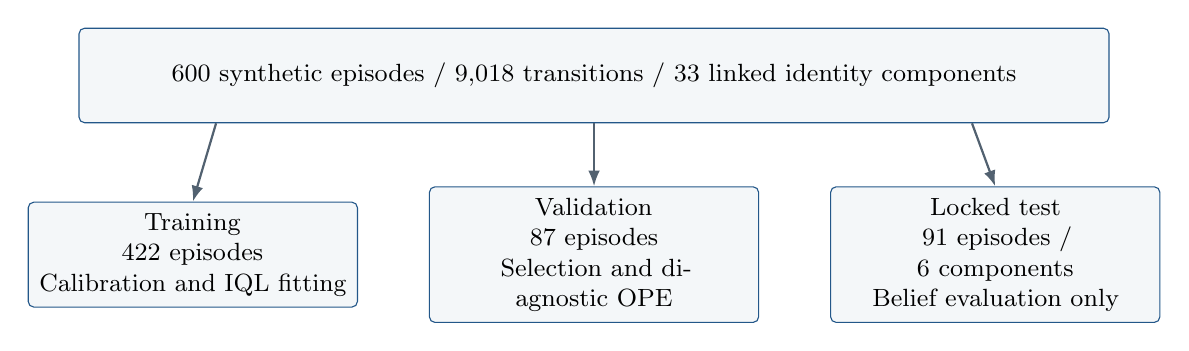
\begin{tikzpicture}[node distance=8mm and 9mm]
\node[box,text width=128mm] (raw) {600 synthetic episodes / 9,018 transitions / 33 linked identity components};
\node[box,below=of raw] (val) {Validation\\87 episodes\\Selection and diagnostic OPE};
\node[box,left=of val] (train) {Training\\422 episodes\\Calibration and IQL fitting};
\node[box,right=of val] (test) {Locked test\\91 episodes / 6 components\\Belief evaluation only};
\draw[arr] (raw.south)--(val.north);
\draw[arr] ([xshift=-48mm]raw.south)--(train.north);
\draw[arr] ([xshift=48mm]raw.south)--(test.north);
\end{tikzpicture}
\caption{Current evaluation partition. Linked identity components remain intact across the split. The locked set is used for the recorded belief comparison, while policy diagnostics use validation transitions.}
\label{fig:split}
\end{figure}

The frozen checkpoint metadata reports seed 42, learning rate $10^{-4}$, target-update coefficient 0.005, patience 10, and best epoch 4. The selected validation objective is 4.13864. This quantity is an optimization statistic, not an interview-performance score. Model identifiers, prompt versions, split assignments, calibration parameters, and checkpoint hashes must accompany a reproduction because a newly generated synthetic corpus is a different experiment.

\subsection{Metrics and comparison rules}
Accuracy measures the fraction of correct classifications. Macro-F1 gives each class equal weight, making it useful when majority classes can dominate accuracy. Balanced accuracy averages class recall. For the belief model, the Brier score assesses the full probability vector, while expected calibration error (ECE) summarizes the difference between confidence and observed correctness in bins. These measures answer different questions; classification accuracy alone does not establish calibrated probabilities \cite{calibration}.

The paired belief comparison applies two frozen configurations to the same 91 episodes. The report resamples identity components to obtain percentile-bootstrap intervals for metric differences. With only six test components, those intervals should be interpreted within the recorded synthetic experiment. The historical module and policy summaries do not provide equivalent paired uncertainty estimates, so numerical differences in those tables are described without claims of statistical significance.

The current policy diagnostic is a normalized importance-weighted average of transition rewards. For logged behavior probability $\mu(a_i\mid s_i)$, its implementation uses
\begin{equation}
\rho_i=\min\left\{\frac{\pi(a_i\mid s_i)}{\mu(a_i\mid s_i)},20\right\},\quad
\widehat R=\frac{\sum_i\rho_i r_i}{\sum_i\rho_i},\quad
\mathrm{ESS}=\frac{(\sum_i\rho_i)^2}{\sum_i\rho_i^2}.
\end{equation}
Because it reweights individual logged transitions, this diagnostic is not a demonstrated estimate of the full discounted return under the target policy's induced state distribution. A favorable value cannot replace fresh rollouts or a justified trajectory-level evaluation protocol.

\section{Baseline results and analysis}
\subsection{Visual and acoustic baselines}
The detailed component report records FER2013 accuracy of 0.5548 and macro-F1 of approximately 0.48 for the CNN. RAVDESS accuracy is 0.5590 and macro-F1 approximately 0.52 for the deep audio model. These values establish useful starting points, but aggregate performance hides uneven class behavior. The visual report lists disgust recall of 0.13, compared with happy recall of 0.80. The acoustic report lists happy recall of 0.10 and disgust recall of 0.89. Such variation argues against mapping an uncertain class prediction directly into a skill judgment.

The separate rapid-run report gives CNN accuracy of 0.5552 and macro-F1 of 0.4600. It also includes deeper architectures trained for much shorter durations. These are retained as another recorded run in Appendix~\ref{sec:rapid}, rather than averaged with the detailed report. A future controlled comparison needs the same examples, preprocessing, stopping rule, and declared compute budget. Without those controls, a lower transformer score can reflect the experiment's budget rather than an inherent weakness of the architecture.

\subsection{Text grading baselines}
Table~\ref{tab:text} contains the five text baselines from the detailed report. The hybrid semantic-rubric model has the highest recorded accuracy, 0.7516, while TF-IDF with a linear SVM has the highest macro-F1, 0.6030. Their accuracy difference is only 0.0021, or 0.21 percentage points. The SVM exceeds the hybrid model's macro-F1 by 0.0144. The preferred model therefore depends on whether the priority is aggregate correctness or balance across the three classes.

\begin{table}[htbp]
\centering\small
\caption{Recorded Mohler text baselines. Precision and recall are supplied at two-decimal resolution; F1 and accuracy retain the report's precision. Bold values mark column maxima within this table only.}
\label{tab:text}
\begin{tabularx}{\linewidth}{p{25mm}YYYY}
\toprule Model & Precision & Recall & Macro-F1 & Accuracy \\ \midrule
TF-IDF + logistic regression & 0.50 & \textbf{0.61} & 0.5167 & 0.6681 \\
TF-IDF + linear SVM & 0.62 & 0.59 & \textbf{0.6030} & 0.7495 \\
SBERT cosine threshold & 0.46 & 0.48 & 0.4629 & 0.6791 \\
SBERT feature classifier & 0.52 & 0.58 & 0.5410 & 0.7165 \\
Hybrid semantic-rubric & \textbf{0.78} & 0.55 & 0.5886 & \textbf{0.7516} \\
\bottomrule
\end{tabularx}
\source{\texttt{ARIA\_updated.md}, Section 10. Results are repository-reported; prediction files and the exact split manifest were not recovered in this revision.}
\end{table}

The dataset summary contains 1,639 expert, 554 intermediate, and 80 beginner examples. This imbalance makes a single accuracy figure particularly difficult to interpret. The stronger SVM macro-F1 is a reason to keep the lexical baseline in subsequent evaluation, not evidence that semantic embeddings are generally inferior. Question-grouped splitting and class-level errors should be recovered before drawing broader conclusions about transfer to unseen interview questions.

\subsection{Does multimodal fusion improve the baseline?}
The CMU-MOSEI ablation provides a direct check on the assumption that combining channels helps. Text-only accuracy is 0.8015, compared with 0.7976 for early fusion, 0.6098 for audio-only, and 0.5808 for vision-only. Fusion is lower than text-only by 0.0039, or 0.39 percentage points. No paired significance test is available, so the result supports a modest conclusion: the recorded experiment does not demonstrate an accuracy gain from early fusion.

\begin{figure}[htbp]
\centering
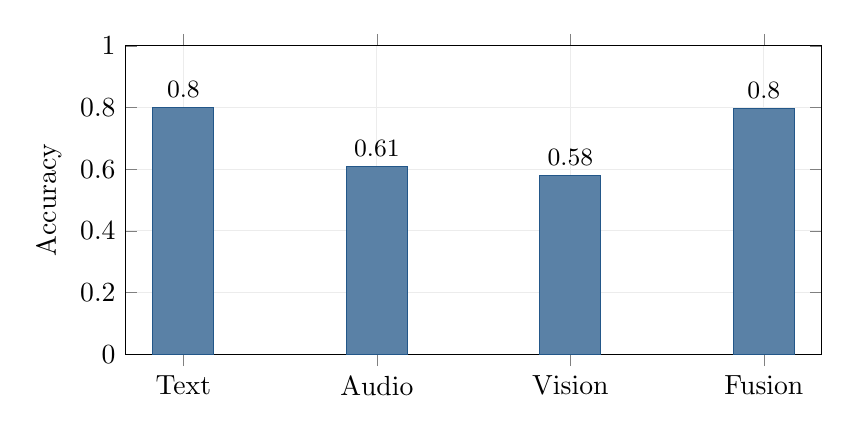
\begin{tikzpicture}
\begin{axis}[width=.86\linewidth,height=5.5cm,ybar,bar width=22pt,ymin=0,ymax=1,ylabel={Accuracy},symbolic x coords={Text,Audio,Vision,Fusion},xtick=data,grid=major,grid style={gray!15},nodes near coords,nodes near coords style={font=\small},point meta=y,ytick={0,.2,.4,.6,.8,1}]
\addplot[fill=ariaBlue!75,draw=ariaBlue] coordinates {(Text,0.8015) (Audio,0.6098) (Vision,0.5808) (Fusion,0.7976)};
\end{axis}
\end{tikzpicture}
\caption{Repository-reported CMU-MOSEI modality ablation. The axis starts at zero to show the small text--fusion difference in context. Uncertainty bars are omitted because the report supplies no run-level or paired uncertainty estimates.}
\label{fig:fusion}
\end{figure}

This finding concerns early concatenation with a classifier. It does not establish that all fusion methods are ineffective. It does, however, set a concrete requirement for a more elaborate model: it should improve on the text-only baseline under a matched protocol. The rapid-run fusion variants all report accuracy of 0.7800 but macro-F1 of 0.4382. Identical aggregate metrics are insufficient to diagnose their prediction behavior; the confusion matrices would be needed before concluding that they learned similar representations or collapsed to a majority class.

\subsection{Annotated incongruence experiment}
The detailed Box of Lies report records accuracy of 0.5965 on a 57-sample test set and reports that the best test accuracy occurred at epoch 2. It also describes training accuracy reaching 1.0 while later test performance remained lower. These observations suggest that model selection and overfitting need closer examination. If the final checkpoint was chosen by repeatedly inspecting test accuracy, that test set would no longer provide an untouched generalization estimate.

The rapid-run report lists accuracy of 0.6800 and macro-F1 of 0.5614 for a multimodal transformer, but the corresponding full training and split artifacts were not located. This remains a recorded exploratory result. In particular, it cannot justify inferring dishonesty from a candidate's facial behavior, accent, or hesitation. The benchmark's annotation target and the intended interview use would require separate validation.

\subsection{Historical policy baselines}
Table~\ref{tab:policy} restores the five-policy comparison already present in the repository. The source describes 300 simulated episodes. It does not provide enough recovered execution detail to confirm pairing, seeds, uncertainty, or equivalence to the present environment. The policy named ARIA in that report is a reward heuristic, not the frozen IQL checkpoint.

\begin{table}[htbp]
\centering\small
\caption{Historical simulation baselines, reported as a 300-episode study. These values must not be interpreted as current IQL rollout results.}
\label{tab:policy}
\begin{tabularx}{\linewidth}{Yrrrrr}
\toprule Policy & Turns & Entropy & Info. gain & Reward & Skill acc. \\ \midrule
Random & 6.77 & 1.4316 & 0.2621 & $-1.1559$ & 0.4933 \\
Fixed script & 10.00 & 1.2792 & 0.4104 & $-1.4683$ & 0.6393 \\
Rule-based adaptive & 19.00 & 1.0865 & 0.7407 & $-1.6446$ & 0.6320 \\
Greedy entropy & 19.00 & 1.4103 & 0.6264 & $-2.0814$ & 0.4767 \\
ARIA reward heuristic & 19.00 & 1.0531 & 0.7666 & $-1.6901$ & 0.6887 \\
\bottomrule
\end{tabularx}
\source{\texttt{ARIA\_updated.md}, Section 10, Model 6. Entropy units and the aggregation definition of skill accuracy are not established by the recovered table.}
\end{table}

The reward heuristic has the highest recorded skill accuracy and information gain, as well as the lowest final entropy. It also uses more turns than the random and fixed-script policies. Random selection has the highest reward because its value is the least negative. Thus, no policy dominates all reported objectives. A plausible concern is that reward and assessment quality are not sufficiently aligned, but the table alone does not identify the cause. Re-running the policies under the current reward definition would test whether the discrepancy persists.

\subsection{Same-data offline-policy comparators}
We trained three additional policies on the frozen v7 development transitions: an MLP behavior-cloning baseline, a discrete CQL adaptation \cite{cql}, and a return-conditioned causal Transformer adapted from Decision Transformer \cite{decisiontransformer}. These are compact ARIA-specific implementations rather than executions of the authors' original code. All use the same 33-dimensional state, eight masked actions, training split, validation split, and seed. The existing IQL checkpoint and generated dataset were not modified. Model selection used validation logged-action accuracy, which was 0.2975 for behavior cloning, 0.2776 for CQL, and 0.1516 for Decision Transformer. This diagnostic measures agreement with logged actions; it is not a rollout performance measure.

Each selected policy was then evaluated on 45 matched synthetic development scenarios, with 15 scenarios per class. The base condition uses separated semantic-score centers. Three prespecified stress conditions increase score overlap, reduce evaluator and modality confidence, or add a positive score shift. Table~\ref{tab:directpolicy} reports assessment accuracy together with the designed cumulative reward and information gain. Bootstrap intervals and episode-level traces are retained in the machine-readable companion reports.

\begin{table}[htbp]
\centering\scriptsize
\caption{Direct learned-policy comparison on matched synthetic development scenarios. Cells show accuracy / mean designed reward / mean information gain. These are not locked-test or human-interview results.}
\label{tab:directpolicy}
\begin{tabularx}{\linewidth}{Yrrrr}
\toprule Policy & Base & Overlap & Low confidence & Positive shift \\ \midrule
ARIA IQL v7 & 1.0000 / 32.16 / 17.88 & 0.4667 / 31.09 / 17.26 & 0.9111 / 11.50 / 3.96 & 1.0000 / 31.14 / 17.27 \\
Behavior cloning & 1.0000 / 25.90 / 14.02 & 0.5333 / 24.28 / 13.01 & 0.9333 / 8.33 / 2.85 & 1.0000 / 25.08 / 13.47 \\
Discrete CQL & 1.0000 / 27.54 / 16.72 & 0.5111 / 25.38 / 15.79 & 0.8889 / 5.01 / 3.35 & 1.0000 / 27.31 / 16.55 \\
Decision Transformer & 1.0000 / 7.22 / 5.13 & 0.4889 / 7.12 / 5.06 & 0.8889 / 2.97 / 1.82 & 1.0000 / 7.04 / 5.01 \\
\bottomrule
\end{tabularx}
\source{Generated comparator and rollout companion reports; all conditions use seed 42. The locked test was not used.}
\end{table}

Base accuracy is a ceiling result: random-valid and fixed-script policies also reach 1.0, so it cannot rank policies. The overlap condition removes that ceiling and reveals no classification winner for IQL; behavior cloning is numerically higher, and the bootstrap intervals overlap. In contrast, IQL has the largest mean designed reward and information gain among the learned comparators in all four conditions and covers all 17 skills. Its paired mean reward advantage over behavior cloning is 6.25 in the base condition (95\% bootstrap interval [5.96, 6.53]) and 6.80 under overlap ([6.35, 7.21]). These findings show alignment with ARIA's simulator reward and exploration objective. Because that reward is designed by the system authors, the result does not independently establish assessment validity or interview quality.

\section{Current locked belief results and policy diagnostic}
\subsection{Paired belief comparison}
The locked JSON report confirms 83 correct predictions out of 91 for the current configuration, compared with 72 out of 91 for the preceding configuration. Macro-F1 rises from 0.8010 to 0.9168. Table~\ref{tab:belief} preserves both favorable and unfavorable changes. The largest class-sensitive change is minimum recall, which increases from 0.5143 to 0.8286.

\begin{table}[htbp]
\centering\small
\caption{Current v7 versus preceding v6 calibration on the same locked synthetic episodes. Arrows indicate the preferred direction.}
\label{tab:belief}
\begin{tabularx}{\linewidth}{Yrrr}
\toprule Metric & v6 & v7 & Difference \\ \midrule
Accuracy $\uparrow$ & 0.7912 & 0.9121 & $+0.1209$ \\
Macro-F1 $\uparrow$ & 0.8010 & 0.9168 & $+0.1158$ \\
Balanced accuracy $\uparrow$ & 0.8179 & 0.9227 & $+0.1048$ \\
Minimum class recall $\uparrow$ & 0.5143 & 0.8286 & $+0.3143$ \\
ECE $\downarrow$ & 0.0808 & 0.0870 & $+0.0062$ \\
Brier score $\downarrow$ & 0.2451 & 0.1395 & $-0.1055$ \\
Ordinal MAE $\downarrow$ & 0.2088 & 0.0879 & $-0.1209$ \\
\bottomrule
\end{tabularx}
\source{\texttt{locked\_test\_evaluation\_v1.json}; 91 episodes, six identity components. Differences are computed from unrounded values.}
\end{table}

The paired component-bootstrap 95\% interval is [0.0435, 0.2235] for the accuracy difference and [0.0443, 0.1976] for the macro-F1 difference. These positive intervals support improvement within this synthetic test. They do not quantify uncertainty for a population of real candidates. ECE increases slightly while the Brier score falls. Reporting only the better classification metrics would conceal this calibration trade-off.

\begin{figure}[htbp]
\centering
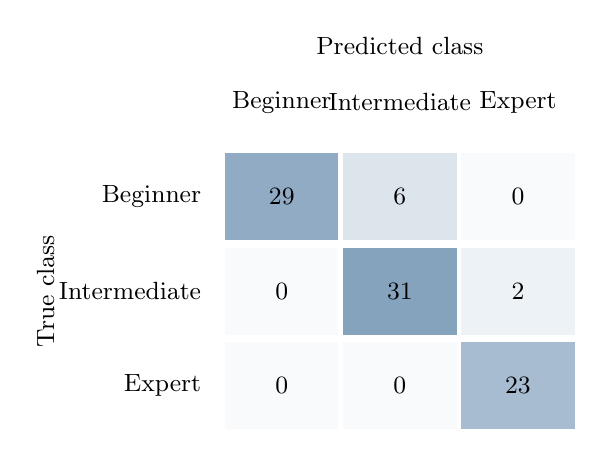
\begin{tikzpicture}[x=15mm,y=12mm,font=\small]
\foreach \x/\name in {0/Beginner,1/Intermediate,2/Expert}{\node at (\x,3.0) {\name};}
\foreach \y/\name in {2/Beginner,1/Intermediate,0/Expert}{\node[anchor=east] at (-.6,\y) {\name};}
\foreach \x/\y/\n/\shade in {0/2/29/50,1/2/6/16,2/2/0/3,0/1/0/3,1/1/31/55,2/1/2/8,0/0/0/3,1/0/0/3,2/0/23/40}{\fill[ariaBlue!\shade] (\x-.48,\y-.46) rectangle (\x+.48,\y+.46);\node at (\x,\y) {\n};}
\node at (1,3.6) {Predicted class};\node[rotate=90] at (-2.0,1) {True class};
\end{tikzpicture}
\caption{Current locked-test confusion matrix. Rows sum to 35, 33, and 23 episodes. Six beginner episodes are predicted as intermediate, and two intermediate episodes as expert. The report's additional abstention column contains zeros and is omitted here.}
\label{fig:confusion}
\end{figure}

All eight mistakes are adjacent-class overestimates. Perfect expert recall therefore does not imply equally strong recognition of all classes. Beginner recall remains the lowest at 0.8286. This asymmetry is relevant when deciding how cautiously the system should interpret weak evidence, and it motivates retaining class-level reporting even when overall accuracy is high.

\subsection{What the policy diagnostic establishes}
The validation diagnostic uses 1,405 transitions and yields a weighted reward estimate of 0.4618. Its effective sample size is 1003.5, the maximum importance ratio is 5.464, and no ratio exceeds the clipping threshold of 20. These values describe the weighting behavior of the available log. They do not demonstrate improved coverage, shorter interviews, or higher assessment quality under the learned policy.

The report explicitly sets the policy release gate to false. The new matched rollouts address policy behavior only in controlled development simulations; they do not change that release decision. The locked belief report, in turn, explicitly states that it does not evaluate the learned policy. This separation resolves an otherwise tempting but invalid inference: the 0.9121 belief accuracy cannot be placed in a policy table as an IQL rollout-accuracy result. The underlying populations, trajectories, and evaluation targets differ.

\section{Discussion}
\subsection{What the baseline results change}
The component results favor a restrained interpretation of architectural complexity. The text experiment gives a simple lexical classifier the strongest macro-F1, and the modality ablation does not show a gain from early fusion. These findings make the baselines part of the argument rather than a formality. The next model should justify additional parameters or sensing requirements through a matched improvement in the target outcome.

The matched comparison confirms that more informative interviews can be longer and that reward ordering can disagree with accuracy ordering. In the overlap condition, IQL collects the most information and reward but has lower accuracy than behavior cloning, CQL, and the uncertainty heuristic. A single scalar reward therefore hides a material trade-off. The present reports retain accuracy, macro-F1, coverage, duration, information gain, reward, bootstrap intervals, and paired initial conditions. Repeated training seeds and an externally justified outcome remain necessary before claiming policy superiority.

\subsection{Relation to contemporary systems}
The SOTA analysis identifies complementary strengths rather than a universal winner. Interactive platforms evaluate question relevance and feedback, predictive models evaluate labels, fairness-aware systems examine group effects, and adaptive testing evaluates selection strategies. ARIA contributes a transparent connection between a calibrated belief representation and an offline action interface. It has not yet reproduced the external studies or evaluated itself on their datasets.

This position also defines a useful route forward. External interview data with a defensible label construction could test the semantic and belief components. A controlled simulator study could test policy behavior. An accessible human practice study could test whether the interaction is understandable and useful. Each study would add a different kind of evidence; one high benchmark score would not replace the others.

\subsection{Limitations and reproducibility}
The current belief evidence is synthetic and clustered into few test components. Its labels reflect the generation and evaluation process rather than independent judgments of real-world competence. The component results are preserved in summary documents, but some raw logs, split manifests, and training scripts referenced by those documents were not recovered. The rapid-run comparison also allocates unequal training time. These limitations prevent claims of broad model superiority.

There are additional use-specific boundaries. Speech-emotion data cannot establish cognitive-load recognition, and annotated deception data cannot establish reliable integrity assessment in interviews. No human criterion-validity, subgroup fairness, or accessibility study has been completed for ARIA. The live application does not execute the evaluated offline stack. These are separate gaps: fixing the application wiring would not validate the measurements, and validating a component would not prove the policy beneficial.

The versioned state schema, frozen JSON reports, comparator checkpoint hashes, policy provenance checks, and deterministic stress conditions provide a basis for reproduction of the current offline release. The direct comparisons are development experiments because the existing locked set had already been used for belief-model analysis before the comparator protocol was defined. For the component studies, the priority is to recover the original predictions and split assignments, resolve the model-name conflicts, and document how checkpoints were selected. Appendix~\ref{sec:provenance} lists the specific distinctions retained in this revision.

\section{Conclusion}
ARIA provides a research architecture for connecting role-grounded mock interviews to calibrated skill beliefs and offline action selection. The recovered baseline results show that simple text models remain competitive and that early multimodal fusion does not automatically improve accuracy. The historical simulation illustrates trade-offs between interview length, information gain, assessment accuracy, and reward.

The current locked experiment supplies the strongest traceable classification evidence: the v7 belief configuration improves accuracy and macro-F1 over v6 on the same 91 synthetic episodes, while ECE shows a small adverse change. The new same-data policy comparison adds a narrower result. IQL consistently obtains the greatest designed reward and information gain among the learned comparators, but it does not lead accuracy when semantic evidence overlaps. The base accuracy of 1.0 is a simulator ceiling rather than evidence of superiority. These findings establish behavior within the specified synthetic protocol; they do not establish real-candidate effectiveness or the validity of automated hiring decisions. A preregistered external evaluation, repeated training seeds, and human validation are the next steps needed to extend the claims.

\appendix
\section{Exploratory 25-model benchmark record}\label{sec:rapid}
Table~\ref{tab:rapid} transcribes the separate rapid-run report. Architecture names are source labels; they were not independently verified against the absent training implementations. Timing is reported execution time, not a standardized measure of inference latency. The baseline and rapid variants should not be ranked as though they received equal training.

\small
\begin{longtable}{p{26mm}p{67mm}rrr}
\caption{Repository-reported rapid-run benchmark matrix. Unequal budgets and unrecovered split details prevent a controlled SOTA ranking.}\label{tab:rapid}\\
\toprule Domain & Architecture & Accuracy & Macro-F1 & Time (s) \\ \midrule
\endfirsthead
\toprule Domain & Architecture & Accuracy & Macro-F1 & Time (s) \\ \midrule
\endhead
\bottomrule\endfoot
Video & Baseline CNN & 0.5552 & 0.4600 & 276.75 \\
Video & ResNet-18 & 0.1800 & 0.0436 & 7.49 \\
Video & MobileNet-SE & 0.2500 & 0.0571 & 5.41 \\
Video & ConvNeXt & 0.1600 & 0.0745 & 5.51 \\
Video & Vision Transformer (ViT) & 0.1700 & 0.0484 & 5.36 \\
Audio & Baseline BiGRU & 0.5590 & 0.5200 & 952.45 \\
Audio & Temporal ConvNet (TCN) & 0.1000 & 0.0227 & 5.52 \\
Audio & Audio Spectrogram Transformer & 0.2800 & 0.1891 & 5.28 \\
Audio & ECAPA-TDNN & 0.2600 & 0.1449 & 5.01 \\
Audio & DenseNet-BiLSTM & 0.1400 & 0.0445 & 5.16 \\
Text & Baseline MLP & 0.6681 & 0.5167 & 54.53 \\
Text & DistilBERT Bi-Encoder & 0.0333 & 0.0215 & 15.03 \\
Text & Gradient Boosted Trees & 0.7833 & 0.5201 & 1.57 \\
Text & Cross-Encoder Network & 0.6167 & 0.3637 & 13.82 \\
Text & BiLSTM Attention & 0.6167 & 0.2543 & 15.00 \\
Fusion & Baseline Early Concat & 0.7976 & 0.7700 & 175.27 \\
Fusion & Tensor Fusion Network & 0.7800 & 0.4382 & 38.79 \\
Fusion & Gated Multimodal Unit & 0.7800 & 0.4382 & 26.94 \\
Fusion & Cross-Modal Transformer & 0.7800 & 0.4382 & 50.75 \\
Fusion & Hierarchical Residual Fusion & 0.7800 & 0.4382 & 39.68 \\
Annotated deception & Baseline Gated Cross-Attention & 0.5965 & 0.5113 & 21.66 \\
Annotated deception & Cross-Modal Dual Attention & 0.6400 & 0.3902 & 13.95 \\
Annotated deception & Multimodal Transformer & 0.6800 & 0.5614 & 13.87 \\
Annotated deception & Multimodal Gradient Boosting & 0.6400 & 0.5322 & 1.75 \\
Annotated deception & Bilinear Tensor Interaction & 0.6400 & 0.3902 & 13.80 \\
\end{longtable}
\normalsize

\section{Provenance and unresolved record differences}\label{sec:provenance}
\begin{table}[htbp]
\centering\small
\caption{Evidence handling for this manuscript revision. These differences remain explicit rather than being silently reconciled.}
\begin{tabularx}{\linewidth}{p{28mm}YY}
\toprule Record & Issue & Treatment \\ \midrule
Detailed component report & FER2013 accuracy 0.5548, macro-F1 about 0.48 & Retained as the detailed-run result \\
Rapid-run report & FER2013 accuracy 0.5552, macro-F1 0.4600 & Retained separately in Appendix A \\
Text model identity & The pair 0.6681/0.5167 is called TF-IDF + logistic regression in one report and baseline MLP in another & No assertion that the two labels identify the same trained model \\
Box of Lies F1 & Detailed report gives rounded 0.55; rapid report gives 0.5113 for the baseline & No pooled F1; only source-specific values retained \\
Historical RL table & Reward heuristic is named ARIA; full rollout artifacts not located & Not relabeled as IQL and not merged with current locked results \\
Current locked evaluation & Machine-readable v6/v7 metrics and hashes are available & Primary numerical evidence for the belief comparison \\
Current OPE & Transition-reward diagnostic; release gate false & Not presented as discounted policy-return improvement \\
Direct policy comparison & Frozen development splits, matched synthetic rollouts, and comparator hashes available & Reported as development-only simulator evidence; locked test not reused \\
\bottomrule
\end{tabularx}
\end{table}

\noindent\textbf{Internal source inventory.} The component and historical-policy tables come from \texttt{ARIA\_updated.md}. Appendix A comes from \texttt{ARIA\_PROJECT\_CONTEXT\_AND\_RESULTS.md}. Current belief results come from \texttt{locked\_test\_evaluation\_v1.json}; the policy diagnostic comes from \texttt{offline\_policy\_evaluation\_v1.json}, both under the production v7 calibration release. Direct comparator summaries, source hashes, and rollout conditions are recorded under \texttt{paper/generated\_sota}. Architecture statements were checked against the state builder, belief update, training code, policy inference module, and application. The companion revision notes preserve exact paths and file hashes.

\begin{thebibliography}{11}
\bibitem{hirenet} L. Hemamou, G. Felhi, V. Vandenbussche, J.-C. Martin, and C. Clavel, ``HireNet: A Hierarchical Attention Model for the Automatic Analysis of Asynchronous Video Job Interviews,'' AAAI, 2019. \url{https://doi.org/10.1609/aaai.v33i01.3301573}. Abstract verified at \url{https://arxiv.org/abs/1907.11062}.
\bibitem{poly} Z. Wen et al., ``PolyInterview: An LLM-based Platform for Immersive Mock Interview Practice with Comprehensive Multimodal Assessment,'' preprint, 2026. \url{https://arxiv.org/abs/2607.10310}.
\bibitem{cat} J. Li, R. Gibbons, and V. Rockova, ``Deep Computerized Adaptive Testing,'' \emph{Psychometrika}, 2026. \url{https://doi.org/10.1017/psy.2026.10106}. Accessible version: \url{https://arxiv.org/abs/2502.19275}.
\bibitem{kim} C. Kim, J. Choi, J. Yoon, D. Yoo, and W. Lee, ``Fairness-Aware Multimodal Learning in Automatic Video Interview Assessment,'' \emph{IEEE Access}, vol. 11, pp. 122677--122693, 2023. \url{https://doi.org/10.1109/ACCESS.2023.3325891}.
\bibitem{mag} B. Putra et al., ``MAG-BERT-ARL for Fair Automated Video Interview Assessment,'' \emph{IEEE Access}, vol. 12, pp. 145188--145205, 2024. \url{https://doi.org/10.1109/ACCESS.2024.3473314}.
\bibitem{avi} T. Zhang, J. Shang, A. Koutsoumpis, Y. Zong, R. E. de Vries, and W. Zheng, ``AVI-Personality: A Trait-Activated Multimodal Dataset for Personality and Competency Assessment in Asynchronous Video Interviews,'' preprint, 2026. \url{https://arxiv.org/abs/2608.25316}.
\bibitem{iql} I. Kostrikov, A. Nair, and S. Levine, ``Offline Reinforcement Learning with Implicit Q-Learning,'' preprint, 2021. \url{https://arxiv.org/abs/2110.06169}.
\bibitem{cql} A. Kumar, A. Zhou, G. Tucker, and S. Levine, ``Conservative Q-Learning for Offline Reinforcement Learning,'' \emph{Advances in Neural Information Processing Systems}, vol. 33, 2020. \url{https://proceedings.neurips.cc/paper/2020/hash/0d2b2061826a5df3221116a5085a6052-Abstract.html}.
\bibitem{decisiontransformer} L. Chen et al., ``Decision Transformer: Reinforcement Learning via Sequence Modeling,'' \emph{Advances in Neural Information Processing Systems}, vol. 34, 2021. \url{https://proceedings.neurips.cc/paper_files/paper/2021/hash/7f489f642a0ddb10272b5c31057f0663-Abstract.html}.
\bibitem{ope} P. Thomas, G. Theocharous, and M. Ghavamzadeh, ``High-Confidence Off-Policy Evaluation,'' AAAI, 2015. \url{https://doi.org/10.1609/aaai.v29i1.9541}.
\bibitem{calibration} C. Guo, G. Pleiss, Y. Sun, and K. Q. Weinberger, ``On Calibration of Modern Neural Networks,'' \emph{PMLR}, vol. 70, pp. 1321--1330, 2017. \url{https://proceedings.mlr.press/v70/guo17a.html}.
\end{thebibliography}
\end{document}
